\documentclass[a4paper,12pt]{report}

\usepackage{cmap}
\usepackage[T2A]{fontenc}
\usepackage[utf8]{inputenc}
\usepackage[english,russian]{babel}
\usepackage{listings}
\usepackage{amsmath}
\usepackage{float}
\usepackage{csquotes}
\usepackage{mathtools}

\usepackage{xcolor}
\usepackage{hyperref}

\usepackage{graphicx}
\graphicspath{ {./images/} }

\definecolor{dkgreen}{rgb}{0,0.6,0}
\definecolor{gray}{rgb}{0.5,0.5,0.5}
\definecolor{mauve}{rgb}{0.58,0,0.82}

\lstset{
    language=Python,                 % выбор языка для подсветки (здесь это С)
    basicstyle=\small\sffamily, % размер и начертание шрифта для подсветки кода
    numbers=left,               % где поставить нумерацию строк (слева\справа)
    numberstyle=\tiny,           % размер шрифта для номеров строк
    stepnumber=1,                   % размер шага между двумя номерами строк
    numbersep=5pt,                % как далеко отстоят номера строк от подсвечиваемого кода
    aboveskip=3mm,
    belowskip=3mm,
    showstringspaces=false,
    columns=flexible,
    captionpos=b, 
    basicstyle={\small\ttfamily},
    numbers=left,
    numberstyle=\tiny\color{gray},
    keywordstyle=\color{blue},
    commentstyle=\color{mauve},
    stringstyle=\color{dkgreen},
    breaklines=true,
    breakatwhitespace=true,
    tabsize=3
}

\title{Лабораторная работа №3\\Апериодические сигналы}
\author{Смирнов Никита}
\date{\today}

\begin{document}

\maketitle
\tableofcontents
\listoffigures
\lstlistoflistings

\maketitle

\chapter{Упражнение 3.1}
\section{Пример утечки}

В данном упражнении нам нужно открыть \texttt{chap01.ipynb}, прочитать пояснения и  запустить примеры. Поэтому я просто изучил все примеры с комментариями. \\ Также нужно заменить окно Хэмингтона одним из окон, предосталяемых NumPy и посмотреть, как они влияют на утечку. Заменим окно Хэмминга.

\begin{lstlisting}[caption=Создание других окон]
for window_func in [np.kaiser, np.bartlett]:
    wave = signal.make_wave(duration)
    if window_func.__name__ == "kaiser":
        wave.ys *= window_func(len(wave.ys), 8)
    else:
        wave.ys *= window_func(len(wave.ys))
    spectrum = wave.make_spectrum()
    spectrum.plot(high=880)
\end{lstlisting}

\begin{figure}[H]
        \centering
        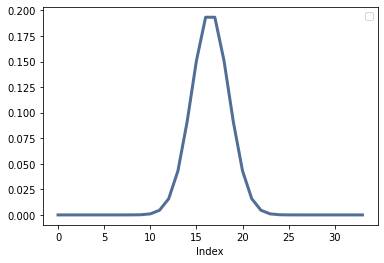
\includegraphics[width=0.75\textwidth]{1.png}
        \caption{Спектр созданных окон}
        \label{fig:lab3_fig1}
\end{figure}

Можно видеть, что окна нормально уменьшают утечку.

\chapter{Упражнение 3.2}
\section{Написание класса SawtoothChirp}

Напишем класс \texttt{SawtoothChirp}, который переопределяет \texttt{evaluate} для генерации пилообразного сигнала.

\begin{lstlisting}[caption=Класс SawtoothChirp]
import math
import thinkdsp

class SawtoothChirp(thinkdsp.Chirp):
    def evaluate(self, ts):
        freqs = np.linspace(self.start, self.end, len(ts) - 1)
        dts = np.diff(ts)
        dphis = (2 * math.pi) * freqs * dts
        phases = np.cumsum(dphis)
        phases = np.insert(phases, 0, 0)
        frac, _ = np.modf(phases)
        ys = self.amp * frac
        return ys
\end{lstlisting}

\section{Проверка работоспособности}

Теперь проверим наши сегменты.

\begin{lstlisting}[caption=Проверка]
test = SawtoothChirp(start=220, end=440)
wave = test.make_wave(duration=1, framerate=10000)
wave.segment(start=0, duration=0.01).plot()
wave.segment(start=1-0.01, duration=0.01).plot()
\end{lstlisting}
    
\begin{figure}[H]
        \centering
        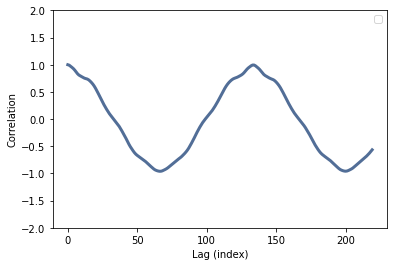
\includegraphics[width=0.75\textwidth]{2.png}
        \caption{Спектр сегмента звука 1}
        \label{fig:lab3_fig2}
\end{figure}

\begin{figure}[H]
        \centering
        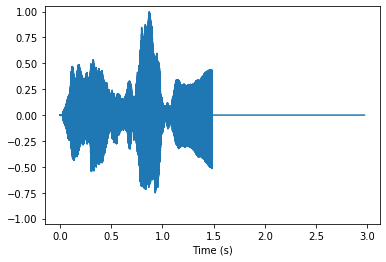
\includegraphics[width=0.75\textwidth]{3.png}
        \caption{Спектр сегмента звука 2}
        \label{fig:lab3_fig3}
\end{figure}

\chapter{Упражнение 3.3}


Создаем сигнал, как просят в задании.

\begin{lstlisting}[caption=Создание сигнала]
signal = SawtoothChirp(start=2500, end=3000)
wave = signal.make_wave(duration=1, framerate=20000)
wave.make_audio()
\end{lstlisting}

Теперь посмотрим на получившийся спектр.

\begin{lstlisting}[caption=Визуализация спектра]
wave.make_spectrum().plot()
\end{lstlisting}

\begin{figure}[H]
        \centering
        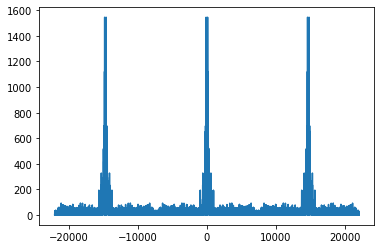
\includegraphics[width=0.75\textwidth]{4.png}
        \caption{Спектр созданного звука}
        \label{fig:lab3_fig4}
\end{figure}


Уберем частоту в самом начале.

\begin{lstlisting}[caption=Удаление частоты в начале]
cut_wave = wave.make_spectrum()
cut_wave.high_pass(10)
cut_wave.plot()
\end{lstlisting}

\begin{figure}[H]
        \centering
        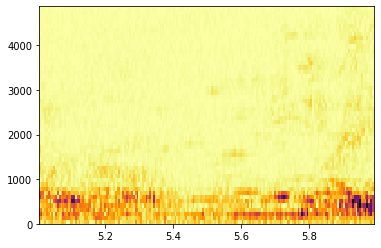
\includegraphics[width=0.75\textwidth]{5.png}
        \caption{Улучшенный спектр созданного звука}
        \label{fig:lab3_fig5}
\end{figure}    

\chapter{Упражнение 3.4}

Для данного задания я взял предложенный вариант файла. 

\begin{lstlisting}[caption=Загрузка и визуализация]
wave = thinkdsp.read_wave('rhapblue11924.wav')
wave.make_audio()
wave.segment(start=1.5, duration=1.8-1.5).plot()
\end{lstlisting}

\begin{figure}[H]
        \centering
        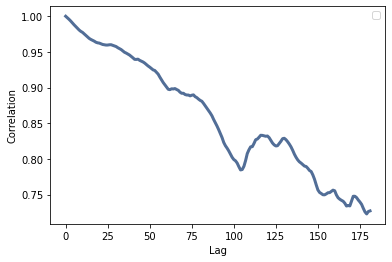
\includegraphics[width=0.75\textwidth]{6.png}
        \caption{Визуализация}
        \label{fig:lab3_fig6}
\end{figure}

Теперь рассмотрим спектр.

\begin{lstlisting}[caption=Спектр]
wave.make_spectrum().plot()
\end{lstlisting}

\begin{figure}[H]
        \centering
        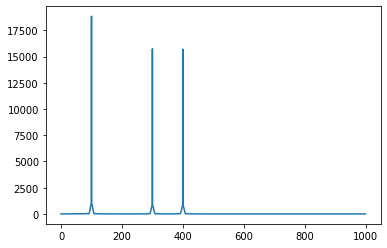
\includegraphics[width=0.75\textwidth]{7.png}
        \caption{Спектр}
        \label{fig:lab3_fig7}
\end{figure}


\chapter{Упражнение 3.5}
\section{Создание класса}

Написанный класс представляет собой тромбоноподобный сигнал с переменной частотой.

\begin{lstlisting}[caption=Создание класса]
class TromboneGliss(thinkdsp.Chirp):
    def _evaluate(self, ts):
        l1, l2 = 1.0 / self.start, 1.0 / self.end
        lengths = np.linspace(l1, l2, len(ts)-1)
        freqs = 1 / lengths
        return self._evaluate(ts, freqs)
\end{lstlisting}

\section{Создание звука и его спектрограмма}

Создадим первую часть звука от C3 до F3, где C3 - 262 Гц, а F3 - 349 Гц.

\begin{lstlisting}[caption=Создание первой части звука]
low = 262
high = 349
signal = TromboneGliss(low, high)
wave1 = signal.make_wave(duration=1)
wave1.apodize()
wave1.make_audio()
\end{lstlisting}

Теперь создадим вторую часть звука от F3 до C3.

\begin{lstlisting}[caption=Создание второй части звука]
signal = TromboneGliss(high, low)
wave2 = signal.make_wave(duration=1)
wave2.apodize()
wave2.make_audio()
\end{lstlisting}

Затем соединим обе части в один полноценный звук.

\begin{lstlisting}[caption=Соединение двух частей звука]
wave = wave1 | wave2
wave.make_audio()
\end{lstlisting}

Теперь сделаем спектрограмму и расммотрим её.

\begin{lstlisting}[caption=Спектрограмма звука]
sp = wave.make_spectrogram(1024)
sp.plot(high=1000)
\end{lstlisting}

\begin{figure}[H]
        \centering
        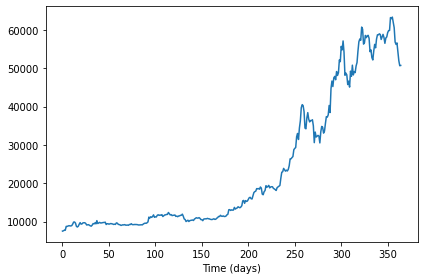
\includegraphics[width=0.75\textwidth]{8.png}
        \caption{Спектрограмма глиссандо на трамбоне}
        \label{fig:lab3_fig8}
\end{figure}


\chapter{Упражнение 3.6}

В интернете я нашёл звуки гласных.

\begin{lstlisting}[caption=Загрузка и прослушивание звука]
wave = thinkdsp.read_wave('Exercise5.2_nasal_dVt.wav')
wave.make_audio()
\end{lstlisting}

Посмотрим на них.

\begin{lstlisting}[caption=Участок]
segment = wave.segment(start=2, duration=5.5)
segment.plot()
\end{lstlisting}

\begin{figure}[H]
        \centering
        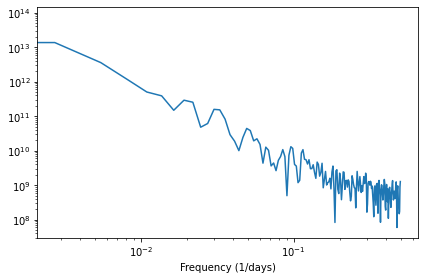
\includegraphics[width=0.75\textwidth]{9.png}
        \caption{Участок}
        \label{fig:lab3_fig9}
\end{figure}


\begin{lstlisting}[caption=Спектограмма]
segment.make_spectrogram(512).plot()
\end{lstlisting}

\begin{figure}[H]
        \centering
        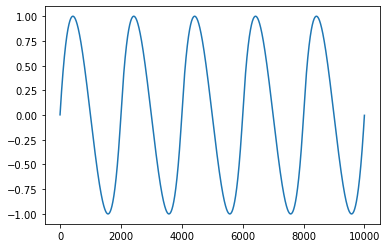
\includegraphics[width=0.75\textwidth]{10.png}
        \caption{Спектограмма}
        \label{fig:lab3_fig10}
\end{figure}

Нам важно то, что некоторые из участков темнее, а некоторые светлее (в рамках одного столбца), что соответствует спектрам соответствующих гласных.


\chapter{Выводы}

Во время выполнения лабораторной работы получены навыки работы с апериодическими сигналами, частотные компоненты которых изменяются во времени, то есть практически все звуковые сигналы. Также рассмотрены спектрограммы - распространённый способ визуализации апериодических сигналов.

\end{document}
